% `template.tex', a bare-bones example employing the AIAA class.
%
% For a more advanced example that makes use of several third-party
% LaTeX packages, see `advanced_example.tex', but please read the
% Known Problems section of the users manual first.
%
% Typical processing for PostScript (PS) output:
%
%  latex template
%  latex template   (repeat as needed to resolve references)
%
%  xdvi template    (onscreen draft display)
%  dvips template   (postscript)
%  gv template.ps   (onscreen display)
%  lpr template.ps  (hardcopy)
%
% With the above, only Encapsulated PostScript (EPS) images can be used.
%
% Typical processing for Portable Document Format (PDF) output:
%
%  pdflatex template
%  pdflatex template      (repeat as needed to resolve references)
%
%  acroread template.pdf  (onscreen display)
%
% If you have EPS figures, you will need to use the epstopdf script
% to convert them to PDF because PDF is a limmited subset of EPS.
% pdflatex accepts a variety of other image formats such as JPG, TIF,
% PNG, and so forth -- check the documentation for your version.
%
% If you do *not* specify suffixes when using the graphicx package's
% \includegraphics command, latex and pdflatex will automatically select
% the appropriate figure format from those available.  This allows you
% to produce PS and PDF output from the same LaTeX source file.
%
% To generate a large format (e.g., 11"x17") PostScript copy for editing
% purposes, use
%
%  dvips -x 1467 -O -0.65in,0.85in -t tabloid template
%
% For further details and support, read the Users Manual, aiaa.pdf.


% Try to reduce the number of latex support calls from people who
% don't read the included documentation.
%
\typeout{}\typeout{If latex fails to find aiaa-tc, read the README file!}
%
\title{•}

\documentclass[]{aiaa-tc}% insert '[draft]' option to show overfull boxes
\usepackage{amsmath}
\usepackage{graphicx}
 \title{Minimum Energy, Reaction Wheel Based, Satellite Attitude Control: A Comparison of Cost Functions}

 \author{
  Dmitriy Rivkin%
    \thanks{Job Title, Department, Address, and AIAA Member Grade.}
  \, 
  Qi Gong\thanksibid{1}
  \, Gabriel Elkaim\thanksibid{1}\\
  {\normalsize\itshape
   University of California Santa Cruz, Santa Cruz, California, 95064, USA}\\
 }

 % Data used by 'handcarry' option if invoked
 \AIAApapernumber{YEAR-NUMBER}
 \AIAAconference{Conference Name, Date, and Location}
 \AIAAcopyright{\AIAAcopyrightD{YEAR}}

 % Define commands to assure consistent treatment throughout document
 \newcommand{\eqnref}[1]{(\ref{#1})}
 \newcommand{\class}[1]{\texttt{#1}}
 \newcommand{\package}[1]{\texttt{#1}}
 \newcommand{\file}[1]{\texttt{#1}}
 \newcommand{\BibTeX}{\textsc{Bib}\TeX}

\begin{document}


\maketitle

\begin{abstract}
This is a bare-bones \LaTeX\ template of an AIAA technical conference paper.
It is intended to demonstrate the bare minimum set of \LaTeX\ commands
to produce an AIAA technical conference paper.
To explore more \LaTeX\ capabilities, see the advanced example, but
first read the Known Problems section of the user manual.
For detailed AIAA layout and style guidelines, please refer to the AIAA
author guide for paper submission, format, and other procedures.
\end{abstract}

\section*{Nomenclature}

\begin{tabbing}
  XXX \= \kill% this line sets tab stop
  $\mathbf{u}$ \> Reaction wheel input torque vector \\
  $\pmb{\omega}$ \> Reaction wheel speed vector \\
  $\pmb{\omega_{B}}$ \> Body angular velocity expressed in body frame\\
  $\mathbf{q}$ \> Unit quaternion representing body frame    orientation \\
  $m$ \> Mass, kg \\
  $\Delta x$ \> Variable displacement vector \\
  $\alpha$ \> Acceleration, m/s\textsuperscript{2} \\[5pt]
  \textit{Subscript}\\
  $i$ \> Variable number \\
 \end{tabbing}

\section{Introduction}

CubeSats operate under severe energy constraints, since their only source of energy is a small covering of solar panels. High performance attitude controllers can increase the capabilities of these small spacecraft, but can use a significant fraction of the energy budget. As such, it is valuable to minimize the energy cost of small satellite attitude maneuvers. We use pseudospectral optimal control methods to compute energy optimal, large angle slew trajectories for a 1U CubeSat using a reaction-wheel-based attitude controller. 

\subsection{Hardware Background}
Reaction-wheel attitude control is based on the principle of momentum exchange between the wheels and the satellite body. When a torque is exerted on a reaction wheel by a motor (usually a brush-less DC motor), the opposite torque is exerted on the satellite body. Three reaction wheels, arranged orthogonally, allow for control in three degrees. This is a popular attitude control method because it does not require any fuel, only electrical energy which can be generated by solar panels.\\

\section{Problem Description}
We are concerned with the computation of a control trajectory for a large angle slew maneuver which minimizes the total electrical energy consumed by the brush-less DC motors that provide actuation torque. The torques exerted by the motors on the wheels are the control variables.We consider three sources of energy consumption. The first are frictional losses, which are proportional to wheel speed squared. The second are resistive losses. The torque produced by an electric motor is proportional to the current flowing through the armature, and energy is dissipated as heat through the resistance of the armature. These losses are proportional to the torque exerted by the motor squared. The third source of energy loss arises when the motor driver is not capable of regenerative braking. This means that any electrical energy converted into mechanical energy by the motor cannot be converted back into electrical energy, and must be dissipated as heat when the wheel slows down. We will hereafter refer to this energy as unrecoverable mechanical energy.   


\section{Methods}
We use Legendre Pseudospectral methods to compute an state-control trajectory pair that minimizes a cost function subject to dynamic constraints, as implemented by the software package DIDO(citation). A similar approach is used in (citations), but we consider a wider variety of cost functions than these papers, which only minimize resistive losses. 

The optimal control solution has an open loop form, and thus requires a closed closed loop controller to track it, such as in Karpenko\cite{Karpenko2014}.


\section{Optimal Control Problem Formulation}

The optimal control problem is formulated as follows:

\begin{align*}
	\text{Minimize} \;\;\; J = 
	\text{Subject to the constraints}: \;\;\; \mathbf{\dot{x}} = \textbf{f}(\textbf{x},\textbf{u}) \\
	\mathbf{x}(t_{0}) = \mathbf{x_{0}}\\
	\mathbf{x}(t_{f}) = \mathbf{x_{f}}\\
	\mathbf{u_{L}} \leq \mathbf{u} \geq \mathbf{u_{U}} 	\\
	\mathbf{x_{L}} \leq \mathbf{x} \geq \mathbf{x_{U}} \\
	t_{0}\text{ and } t_{f} \text{ fixed}
\end{align*}

The dynamic constraints, $\textbf{f}(\textbf{x},\textbf{u})$, can be found in the appendix.\\ 
\\
The cost function $J$ takes on one of the following forms, depending on the optimization being performed.
\begin{align*}
\text{To minimize frictional losses:} \qquad
J = FL = \int_{t_{0}}^{t_{f}} \sum_{i = 1}^{3}\omega_{i}^{2} \; dt \\
\\
\text{To minimize resistive losses:} \qquad
J = RL = \int_{t_{0}}^{t_{f}} \sum_{i = 1}^{3}u_{i}^{2} \; dt \\
\\
\text{To minimize unrecoverable mechanical energy:}\qquad 
J=UM=\int_{t_{0}}^{t_{f}} \sum_{i = 1}^{3}F_{i} \; dt \\
	F_{i}  = \begin{cases}
    \omega_{i}u_{i},& \text{if } \omega_{i}u_{i}\geq 0\\
    0,              & \text{otherwise}
	\end{cases} \\
\end{align*}




\subsection{Cost Function Practical Considerations}
When performing numerical optimization, it is desirable for the cost function to be continuous and smooth. Cost functions $FL$ and $RL$ satisfy these criteria, while cost function $UM$ is non-smooth at zero. Attempting a numerical optimization using $UM$ as the cost function does not yield a satisfying (i.e. feasible). To improve performance, we define an approximate cost function, $\hat{UM}$which is smooth on the interval ($-\infty , +\infty$).

\begin{align*}
\hat{UM} = \int_{t_{0}}^{t_{f}} \sum_{i = 1}^{3}\frac{1}{\alpha}ln(1+e^{\alpha \omega_{i} u_{i}}) \; dt, \qquad \alpha > 0 \\
\end{align*}

As the scaling factor, $\alpha$, gets large, $\hat{UM}$ becomes arbitrarily close to $UM$, as illustrated in figure \ref{f:UMhat}.

\begin{figure}[h!]% order of placement preference: here, top, bottom
\centering
 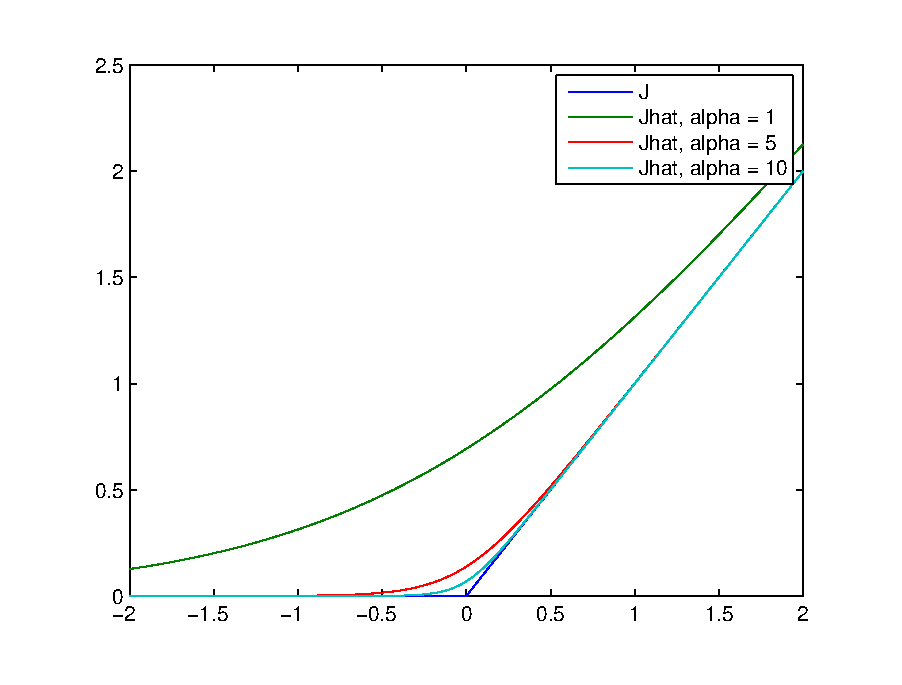
\includegraphics[width = 3in]{cfapprox}
 \caption{Jhat approaches J as alpha gets larger}
 \label{f:UMhat}
\end{figure}

\section{Results}
We present control trajectories for a large angle slew of a 1U CubeSat, whose parameters can be found in the appendix. Table \ref{t:pcomp} provides a comparison of the performance of the three numerical solutions with respect to the three cost functions of interest.

\begin{table}% no placement specified: defaults to here, top, bottom, page
 \begin{center}
  \label{t:pcomp}
  \begin{tabular}{rrrr}
        & $UM$ & $FL$ & $RL$ \\
        $\hat{UM}$ &  1.00 & 1.01 & 5.10 \\
        $FL$ &  1.23 & 1.00 & 11.30 \\
       $RL$ &  2.09 & 1.29 & 1.00 \\
         \end{tabular}
 \end{center}
   \caption{Normalized performance of numerical solutions with respect to different cost functions}
\end{table}

\subsection{Discussion}

     


\section{Conclusion}
The solutions found w.r.t cost functions $FL$ and $\hat{UM}$ are the nearly the same and have Bang-Off-Bang form. On the other hand, the control which optimizes $RL$ is continuous and smooth, making it apparent why the $RL$ cost function is a popular choice for optimization. It also performs reasonably well with respect to $FL$. However, it performs poorly with respect to $UM$, demonstrating that in the absence of regenerative braking, optimizing with respect to $RL$ may not yield a truly energy optimal solution. A better approach would be to optimize a cost function which is a weighted sum of the three, the relative weights being dependent on the specific system at hand. In the full paper, we find a solution of this nature for a commercially available CubeSat attitude controller. 


\section*{Appendix}

Dynamics as derived by Karpenko\cite{Karpenko2014}
\begin{align}
\textbf{f}(\textbf{x},\textbf{u}) = 
\begin{bmatrix}
a\\
b
\end{bmatrix}
\end{align}


\bibliographystyle{AAS_publication}
\bibliography{C:/Users/Dmitriy/Documents/library}



\end{document}

% - Release $Name:  $ -
